\documentclass{article}
\usepackage{graphicx} % Required for inserting images
\usepackage[top=0.9in, bottom=1in, left=1.5in, right=1.5in]{geometry}
\usepackage[utf8]{inputenc}
\usepackage[icelandic]{babel}
\usepackage[T1]{fontenc}
\usepackage[sc]{mathpazo}
\usepackage[parfill]{parskip}
\renewcommand{\baselinestretch}{1.2}
% Tables and lists
\usepackage{booktabs,tabularx}
\usepackage{multirow}
\usepackage{enumerate}
\usepackage{adjustbox}
\usepackage{multicol}
\usepackage{xcolor}
\usepackage{algpseudocode}
\usepackage{tikz}
\usepackage{nicefrac}
\usepackage{changepage}
\usetikzlibrary{arrows, positioning, calc, graphs}

% Math
\usepackage{amsmath, amsfonts, amssymb, amsthm}
% Graphics

\usepackage{graphicx}
\usepackage{tikz}
% Code environment
\usepackage{minted}
%\usepackage{bm}
%\usepackage{siunitx}
%\usepackage{animate}
%\usepackage{hyperref}
%\usepackage{movie15}
%\usepackage{multicol}
%\usepackage{changepage}
\title{Forritunarmál Einstaklingsverkefni 8}
\author{Ragnar Björn Ingvarsson, rbi3}
\tikzset{->, >=stealth', shorten >=1pt, node distance=2cm,thick, main node/.style={circle,draw,minimum size=3em}}

\begin{document}
\renewcommand\thepage{}
	
	\maketitle

	\newpage
	\setcounter{page}{1}
	\renewcommand\thepage{\arabic{page}}

	\section{}
	\begin{verbatim}
;;; Notkun: y = sort(x);
;;; Fyrir:  x er listi talna.
;;; Eftir:  y er listi sem inniheldur sömu gildi
;;;         og x en í vaxandi röð.
rec fun sort(x)
{
    ;;; Notkun: y = insert(x,v);
    ;;; Fyrir:  x er listi talna, v er tala.
    ;;;         x er í vaxandi röð.
    ;;; Eftir:  y er listi í vaxandi röð sem
    ;;;         inniheldur öll gildin í x auk 
    ;;;         gildisins v.
    rec fun insert(x, v)
    {
        if (x == []) { return [v] };
        if (head(x) > v) { return v : x };
        return head(x) : insert(tail(x), v);
    };
    if (x == []) { return x };
    return insert(sort(tail(x)), head(x));
};
	\end{verbatim}
	\begin{center}
		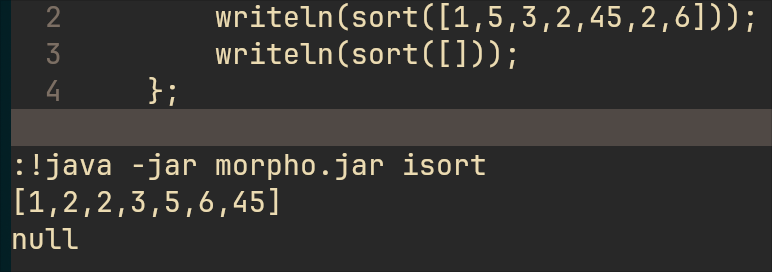
\includegraphics[scale=0.35]{isort.png}
	\end{center}
	Ath. að þegar morpho prentar tóma listann prentast út "null"\hspace{0.1em} svo 
	sort([]) skilar í raun tóma listanum [].

\end{document}
